\section{Experimental setup} As shown in the \cref{fig:Eexperimental_setup} the setup consists of 2 cameras (Kinect by Microsoft and fusionTrac 500 by Atarcsys), A robot (UR3 by Universal Robots), phantom head, multiple EEG caps, 2 markers as shown in \cref{fig:markers} each serving a specific purpose. The purpose of each hardware used is briefly described below.\\

\begin{figure}[hbt!]
	\centering
	\begin{subfigure}{0.49\textwidth}
		\includegraphics[width=\textwidth]{experimental_setup_1.jpg}	
	\end{subfigure}
	\hfill
	\begin{subfigure}{0.49\textwidth}
		\includegraphics[width=\textwidth]{experimental_setup_2.jpg}	
	\end{subfigure}
	\caption{Experimental setup consists of Microsoft kinect, Atracsys fusionTrac 500, UR3 robot.} 
	\label{fig:Eexperimental_setup}
\end{figure} 

\begin{enumerate}
	\item \textbf{Kinect camera} 
	\begin{itemize}
		\item Record information such as robot movement, point cloud data, RGBD images, etc.
	\end{itemize}
	\item \textbf{fusionTrac 500} 
	\begin{itemize}
		\item Head coordinate system creation.
		\item Electrode mapping.
	\end{itemize}
	\item \textbf{UR3} 
	\begin{itemize}
		\item Simulate the patient's head movement.
	\end{itemize}
	\item \textbf{EEG caps} 
	\begin{itemize}
		\item Caps with different electorde patterns are used to generate ground truth data.
	\end{itemize}
	\item \textbf{Chessboard and reflective marker} 
	\begin{itemize}
		\item Hand-eye calibration.
		\item Electrode mapping.
	\end{itemize}
\end{enumerate}

\subsection{Kinect camera} Microsoft azure Kinect camera \cite{azure_kinect} comes with many sophisticated sensors integrated. For example, 12Megapixel RGB sensor, 1 Megapixel time of flight (Tof) depth sensor, motion sensor (accelerometer and gyroscope) and microphone array which provides excellent computer vision and speech models. The camera is compact in size and comes with an USB interface to the computer as shown in \cref{fig:azure_kinect}. Microsoft also provides a software development kit (SDK) and easy to use interface for accessing all the sensors. SDK also provides an interface to the robot operating system (ROS).   

\begin{figure}[hbt!]
	\centering
	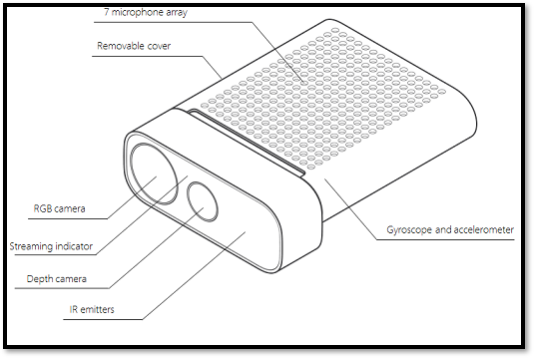
\includegraphics[scale=0.5]{azure_kinect.png}
	\hfill
	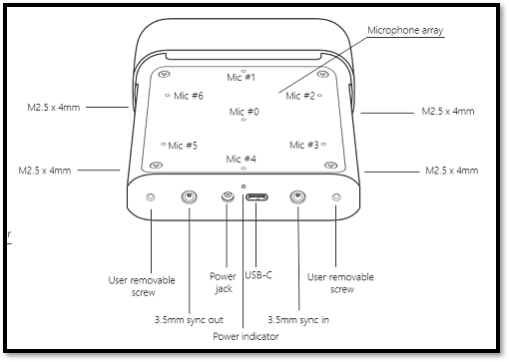
\includegraphics[scale=0.52]{azure_kinect_2.png}
	\caption{Microsoft azure kinect camera features.} 
	\label{fig:azure_kinect}
\end{figure}

 \subsection{fusionTrac 500} The fusionTrac 500 by Atracsys \cref{fig:fusionTrac} is a passive and active, real-time optical pose-tracking system specially designed to detect and track reflective spheres, disks, and IR-LEDs in real-time. The fusionTrack has two cameras that observe reflective and/or active fiducials (IR LEDs) simultaneously, and it triangulates the detected markers to calculate their locations with high precision and a measurement rate of 335 Hz. The fusionTrac system can be used to estimate the pose when several fiducials are arranged to form a specific shape.

\begin{figure}[hbt!]
	\centering
	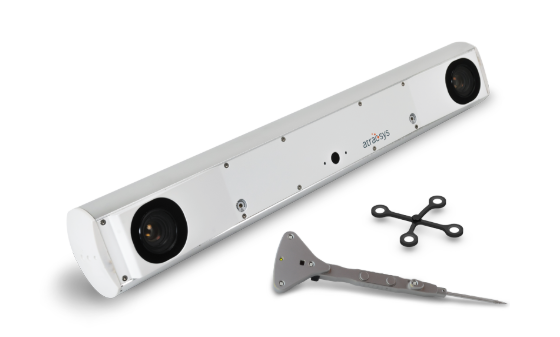
\includegraphics[scale=0.5]{fusionTrac.png}
	\caption{fusionTrac 500 \cite{fustionTrac}} 
	\label{fig:fusionTrac}
\end{figure} 

fusionTrac provides software development kit (SDK) to seamlessly access the data via TCP/IP server and client based system. 

\subsection{UR3 Robot}

To simulate the patient's head movements the phantom head has been mounted to ur3 robot from Universal Robotics \cref{fig:ur3} and moved along predefined trajectories. It comes with an onboard controller and an easy tab interface to control. The robot prevents itself against any unforeseen forces by the operator and the environment. Universal robotics also provides a ROS interface from where the robot can be controlled via scripts. The important specifications of the UR3 robot is given in table \ref{tab:UR3 specification}.

\begin{figure}[hbt!]
	\centering
		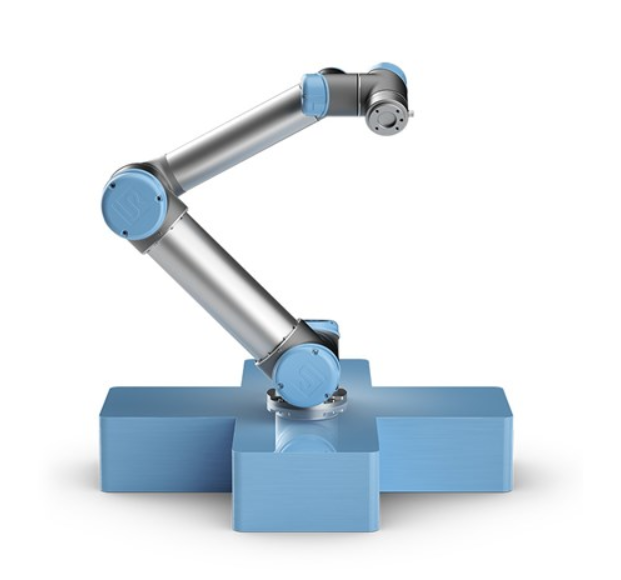
\includegraphics[scale=0.8]{UR3.png}
		\caption{UR3 robot \cite{UR3}}
		\label{fig:ur3}	
\end{figure}

\begin{table}[hbt]
	\centering
	\begin{tabular}{|c|c|}
		\hline
		Specification & UR3\\ 
		\hline
		Repeatability & $\pm$ 0.1 mm\\
		Payload & 3 Kg\\
		Reach & 500mm \\
		Degrees of freedom & 6 rotating joitns\\
		\hline
	\end{tabular}
	\caption{Important specifications of UR3 robot}
	\label{tab:UR3 specification}
\end{table}

\subsection{Phantom head}
In order to simulate the patient's head, a dummy phantom head has been used all through the project as shown in the \cref{fig:Phantom_head}  

\begin{figure}[hbt!]
	\centering
	\begin{subfigure}{0.32\textwidth}
		\includegraphics[width=\textwidth]{phantom_1.jpg}	
	\end{subfigure}
	\hfill
	\begin{subfigure}{0.32\textwidth}
		\includegraphics[width=\textwidth]{phantom_2.jpg}	
	\end{subfigure}
	\hfill
	\begin{subfigure}{0.32\textwidth}
		\includegraphics[width=\textwidth]{phantom_3.jpg}	
	\end{subfigure}
	\caption{Phantom head used in the experiments.} 
	\label{fig:Phantom_head}
\end{figure} 

\subsection{Electode caps}

Several EEG caps provided by eemagine Medical Imaging Solutions GmbH, Berlin, Germany are used to generate the data as shown in \cref{fig:Electrode_caps} and \cref{fig:multiple_eeg_caps}.

\begin{figure}[hbt!]
	\centering
	\begin{subfigure}{0.49\textwidth}
		\includegraphics[width=\textwidth]{electrode_1.jpg}	
	\end{subfigure}
	\hfill
	\begin{subfigure}{0.49\textwidth}
		\includegraphics[width=\textwidth]{electrode_2.jpg}	
	\end{subfigure}
	\caption{EEG cap on the phantom head.} 
	\label{fig:Electrode_caps}
\end{figure} 

\begin{figure}[hbt!]
	\centering
	\includegraphics[width=\linewidth]{different_EEG_caps.jpg}
	\caption{Multiple EEG caps with different elctrode location}
	\label{fig:multiple_eeg_caps}	
\end{figure}

\subsection{Markers}
A Chessboard with grid size (5 $\times$ 8) is used for camera and hand-eye calibration of Kinect while reflective marker is used with fusionTrac 500. Both markers can be seen in the \cref{fig:markers}.  

\begin{figure}[hbt!]
	\centering
	\begin{subfigure}{0.49\textwidth}
		\includegraphics[width=\textwidth]{chessboard.jpg}	
	\end{subfigure}
	\hfill
	\begin{subfigure}{0.49\textwidth}
		\includegraphics[width=\textwidth]{active_marker.jpg}	
	\end{subfigure}
	\caption{Two types of markers used in the experiments, chessboard and active reflective marker} 
	\label{fig:markers}
\end{figure} 